\documentclass{article}
\usepackage[utf8]{inputenc}
\usepackage[spanish]{babel}
\usepackage[document]{ragged2e}
\usepackage{graphicx}
\usepackage{listings}
\usepackage{url}
\usepackage{wasysym}
\usepackage{color}
\usepackage[utf8]{inputenc}
\definecolor{dkgreen}{rgb}{0,0.6,0}
\definecolor{gray}{rgb}{0.5,0.5,0.5}
\definecolor{mauve}{rgb}{0.58,0,0.82}



\lstset{frame=tb,
  language=Python,
  aboveskip=3mm,
  belowskip=3mm,
  showstringspaces=false,
  columns=flexible,
  basicstyle={\small\ttfamily},
  numbers=none,
  numberstyle=\tiny\color{gray},
  keywordstyle=\color{blue},
  commentstyle=\color{dkgreen},
  stringstyle=\color{mauve},
  breaklines=true,
  breakatwhitespace=true,
  tabsize=3
}
\title{Optimización de flujo en redes \linebreak   Tarea 1: Representación de redes a través de la teoría de grafos}

\author{Alberto Martínez Noa \linebreak Matricula-1985271}
\date{\today}

\begin{document}
\maketitle
\section{ Grafo simple no dirigido acíclico}
Se pueden encontrar varias aplicaciones a la modelación de un grafo simple no dirigido acíclico, una de las más claras son los árboles, "el árbol (árbol libre) que es un grafo no dirigido, conexo y acíclico. Un árbol también puede definirse como un grafo no dirigido en el que hay exactamente un camino entre todo par de vértices"\cite{gf1} \linebreak
Un ejemplo de usos de árboles es en topología de red la de árbol, en esta topología los nodos de la red están ubicados en forma de árbol. esta conexión es similar a muchas redes en estrella interconectadas con la diferencia de no poseer un nodo central, en cambio posee un nodo troncal desde el cual se ramifican el resto de los nodos como se muestra en la figura 1 que es una pequeña representación con solo 8 nodos de la red que posee la UEB Rolando Peréz Gollanes entidad dedicada al sacrificio y procesamiento de aves.
 
 
\begin{center}
\lstinputlisting[language=Python]{grafo1.py}
\end{center}
\begin{figure}[h]
\begin{center}
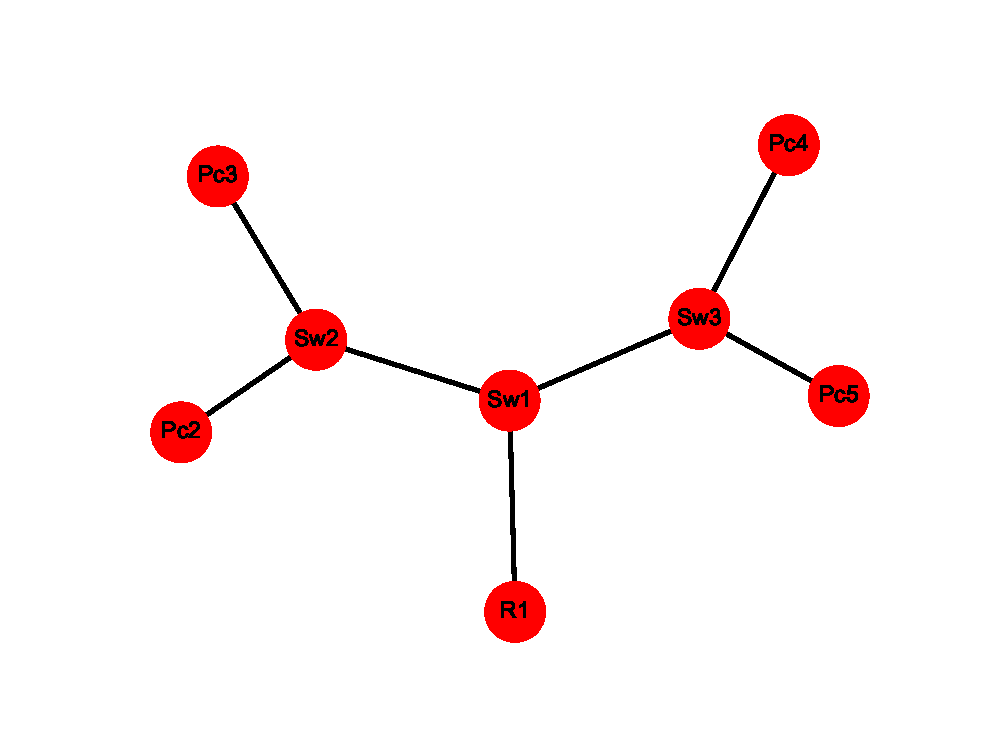
\includegraphics[scale=0.7]{Graf1.eps}\\
\caption{Grafo simple no dirigido acíclico}
\end{center}
\end{figure}

\section{Grafo simple no dirigido cíclico}
Un grafo simple no dirigido cíclico puede usarse áreas como geografía: Si se considera un mapa, digamos de Europa. Que cada país sea un vértice y conecte dos vértices con una arista si esos países comparten una frontera. Un problema famoso que quedó sin resolver durante más de cien años fue el problema de los cuatro colores. Aproximadamente esto indica que cualquier mapa puede ser coloreado con a lo sumo 4 colores de tal manera que los países adyacentes no tengan el mismo color. Este problema motivó muchos desarrollos en la teoría de grafos y finalmente se demostró con la ayuda de una computadora en 1976\cite{rf1}.\linebreak

Otra aplicación es en la representación de redes sociales, una red social se conceptualiza como un grafo, es decir, un conjunto de vértices (o nodos, unidades, puntos) que representan entidades u objetos sociales y un conjunto de líneas que representan una o más relaciones sociales entre ellos\cite {article1}.\linebreak
Por ejemplo, si consideramos un grupo de 9 doctores del núcleo académico de PISIS (Posgrado en Ingeniería de Sistemas) y construimos una red, tomando como vértices a los doctores y la colaboración de ellos en artículos publicados como aristas dará lugar a un grafo simple no dirigido cíclico como se muestra en la figura 2.

    
\begin{center}
\lstinputlisting[language=Python]{grafo2.py}
\end{center}
\begin{figure}[h]
\begin{center}
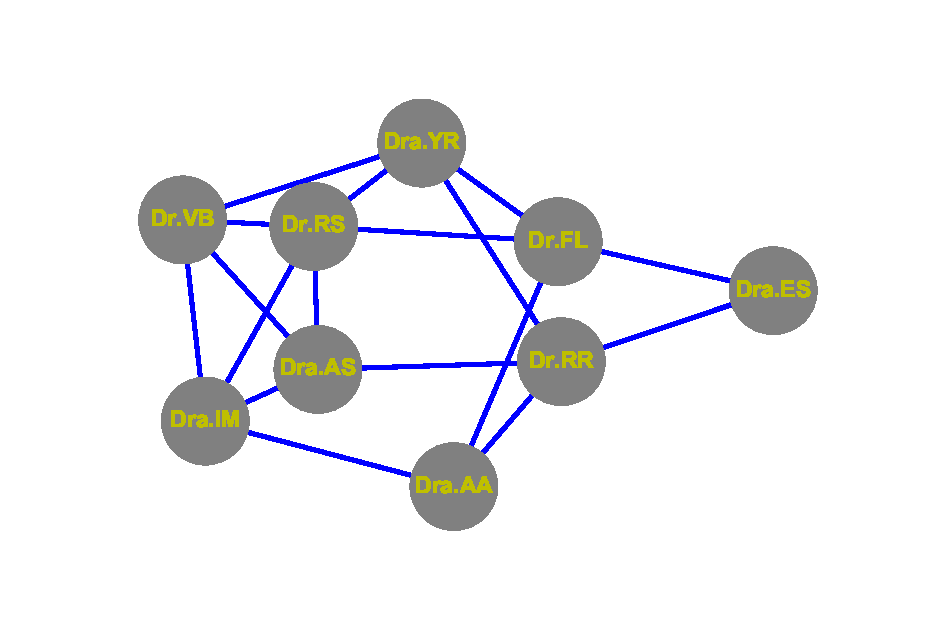
\includegraphics[scale=0.7]{Graf2.eps}\\
\caption{Grafo simple no dirigido cíclico}
\end{center}

\end{figure}


\section{Grafo simple no dirigido reflexivo}
Una de las aplicaciones de este tipo de grafo es en la modelación de comportamientos de elementos sociales en la vida real.\linebreak
Por ejemplo, en un estudio sobre el comportamiento sexual de un grupo de adolescentes con edades comprendida entre 15 y 18 años, se representar las relaciones sexuales consentidas(aristas) que existen entre los individuos(vértices) del grupo, así como la satisfacción, para así saber tendencias por edades, posibles esquemas de propagación de enfermedades y promiscuidad entre otros factores del interés de los sexólogos. Este ejemplo se muestra en el grafo de la figura 3.  
  
\begin{center}
\lstinputlisting[language=Python]{grafo3.py}
\end{center}
\begin{figure}[h]
\begin{center}
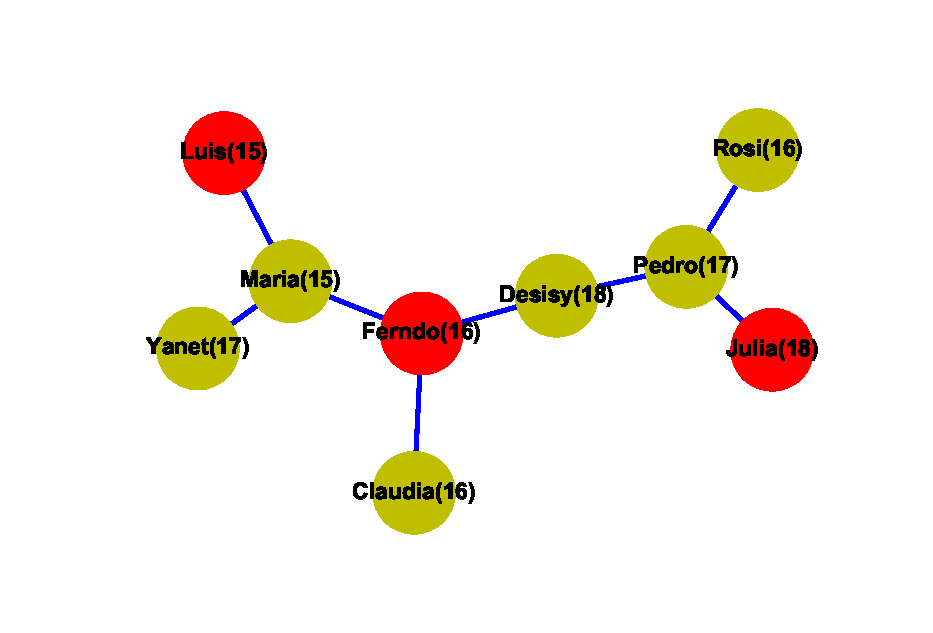
\includegraphics[scale=0.7]{Graf3.eps}\\
\caption{Grafo simple no dirigido reflexivo,donde los vértices rojos representan los nodos donde están las aristas reflexivas}
\end{center}
\end{figure}

\section{Grafo simple dirigido acíclico}
Encontraos entre las aplicaciones de los grafos dirigidos o dígrafos acíclico las siguientes: 
\begin{itemize}
\item Una red bayesiana queda especificada formalmente por una dupla B= (G, O), donde G es un grafo dirigido acíclico (GDA) y O es el conjunto de distribuciones de probabilidad. Definimos un grafo como un par G= (V, E), donde V es un conjunto finito de vértices nodos o variables y E es un subconjunto del producto cartesiano V x V de pares ordenados de nodos que llamamos enlaces o aristas\cite{gf2}.
\item Los arboles dirigidos son un ejemplo clásico de grafos dirigidos acíclico, estos tienen múltiples en la cotidianidad como pueden ser los arbole genealógicos, los organigramas de una empresa (referido a las jerarquías entre los empleados) y el árbol de directorios de Windows.

\end{itemize}	
En la figura 4 se muestra un ejemplo de red bayesiana (topología de red para el cáncer de pulmón), donde C(cáncer), Con(Contaminación), F(Fumador), D(disnea),Rx(rayos-x)son los vértices y sus relaciones son las aristas.

\begin{center}
\lstinputlisting[language=Python]{grafo4.py}
\end{center}

\begin{figure}[h]
\begin{center}
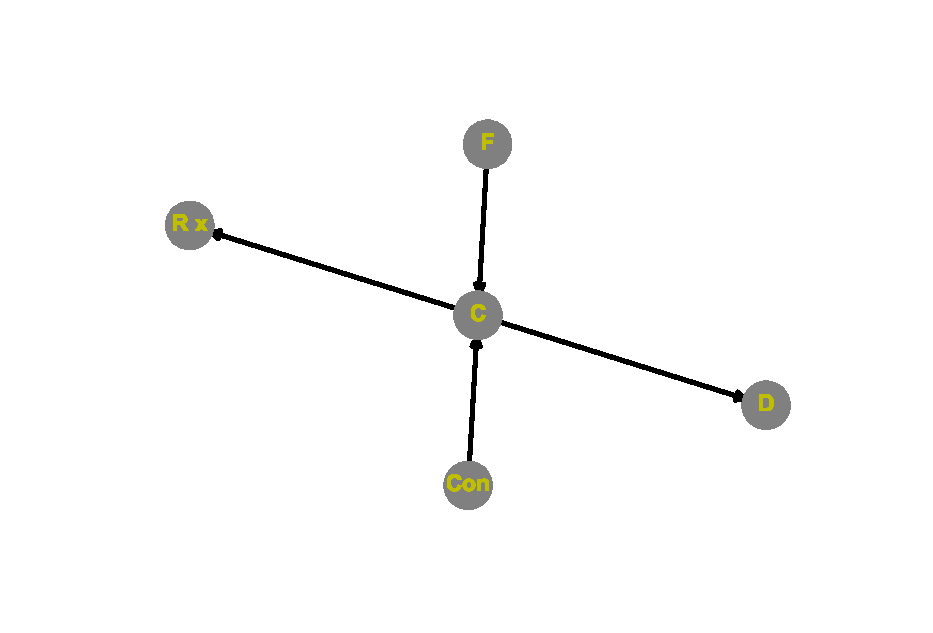
\includegraphics[scale=0.7]{Graf4.eps}\\
\caption{Grafo simple dirigido acíclico}
\end{center}

\end{figure}
\section{Grafo simple dirigido cíclico}
Aplicaciones de los Grafo dirigido cíclico:
\begin{itemize}
\item En ingeniería eléctrica se utilizan grafos dirigidos cíclicos en el análisis de circuito desde Kirchoff en los años 1850.
\item En redes sociales, otro enfoque de redes sociales en su análisis puede arrojar un grafo dirigido cíclico si te tomamos como vértices a personas y como aristas el sentimiento de amistad de una persona hacia otra, este ejemplo se refleja en el grafo de la figura 5.


\end{itemize}
\begin{center}
\lstinputlisting[language=Python]{grafo5.py}
\end{center}

\begin{figure}[h]
\begin{center}
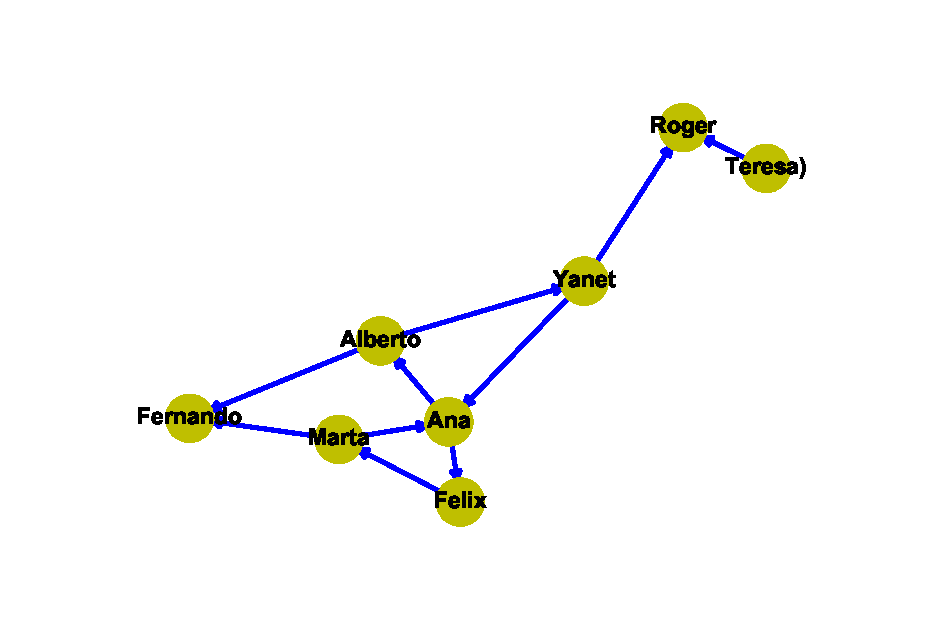
\includegraphics[scale=0.7]{Graf5.eps}\\
\caption{Grafo simple dirigido cíclico}
\end{center}

\end{figure}
\section{Grafo simple dirigido reflexivo}

Las aplicaciones de estos grafos van desde la representación del funcionamiento de las páginas web, el modelado de una empresa de servicio que brinda el mismo tanto a sus clientes como a ella misma, hasta representar un grafo que modele la comprobación de una red de computadoras. \linebreak
Por ejemplo, suponiendo que se está comprobando la conectividad entre los nodos(equipos) de una red de computadoras, es decir que un nodo puede dar ping a cualquier otro nodo, significa que dicho nodo está conectado con el resto, además se debe asegurar que el mismo nodo pueda recibir un auto-ping, si esto no ocurre existe un problema de conectividad. La figura 6 muestra dicho ejemplo.

\begin{center}
\lstinputlisting[language=Python]{grafo6.py}
\end{center}
\begin{figure}[h]
\begin{center}
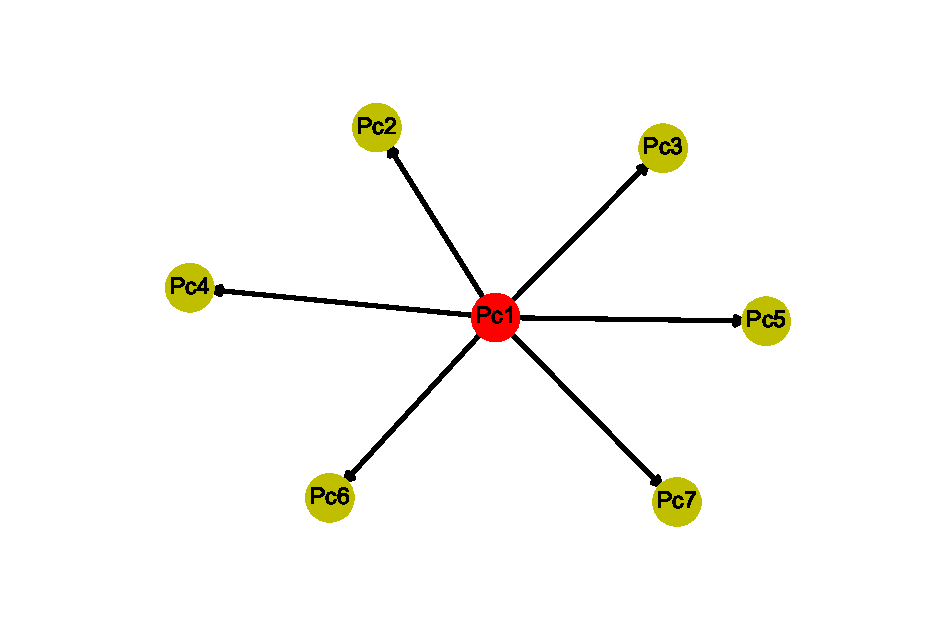
\includegraphics[scale=0.7]{Graf6.eps}\\
\caption{Grafo simple dirigido reflexivo, donde el vértice rojo representa la arista reflexiva}
\end{center}
\end{figure}
 \section{Multigrafo no dirigido acíclico}
Una de las aplicaciones de este tipo de grafo es en el tasado de rutas.
Por ejemplo, considerando que se quiere tranzar los diferentes caminos (sin importar el sentido de estos) que comunican a varios Municipios de La Habana en un orden específico (Lisa, Marianao, Playa, Vedado, Habana Vieja, Habana del Este). Tomando como vértices los municipios y como aristas las carreteras que los unen, esto da lugar al grafo que muestra la figura 7.
\begin{center}
\lstinputlisting[language=Python]{grafo7.py}
\end{center}
\begin{figure}[h]
\begin{center}
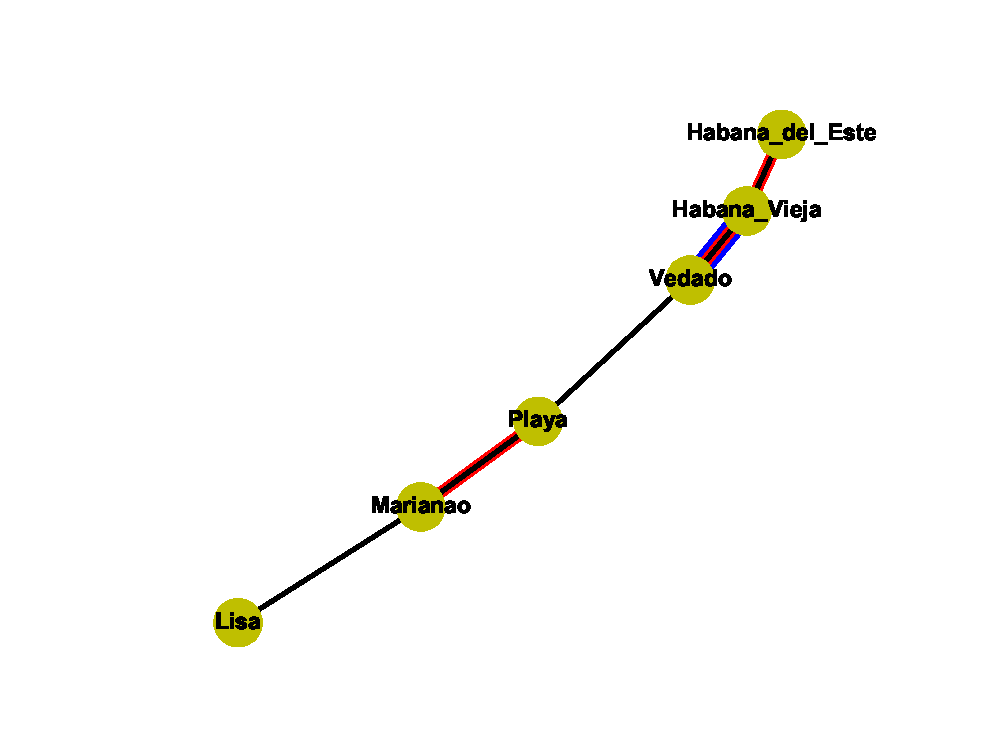
\includegraphics[scale=0.7]{Graf7.eps}\\
\caption{Multigrafo no dirigido acíclico, donde los diferente colores de los arcos representan los diferentes caminos}
\end{center}
\end{figure}
\section{Multigrafo no dirigido cíclico}

Un ejemplo donde podemos utilizar este tipo de grafos es: se quiere representar cuantas llamadas(aristas)se realizaron entre un grupo de personas(vértices), donde nos importa saber la duración de cada llamada durante un día determinado. Este grafo se ve representado en la figura 8.

\begin{center}
\lstinputlisting[language=Python]{grafo8.py}
\end{center}
\begin{figure}[h]
\begin{center}
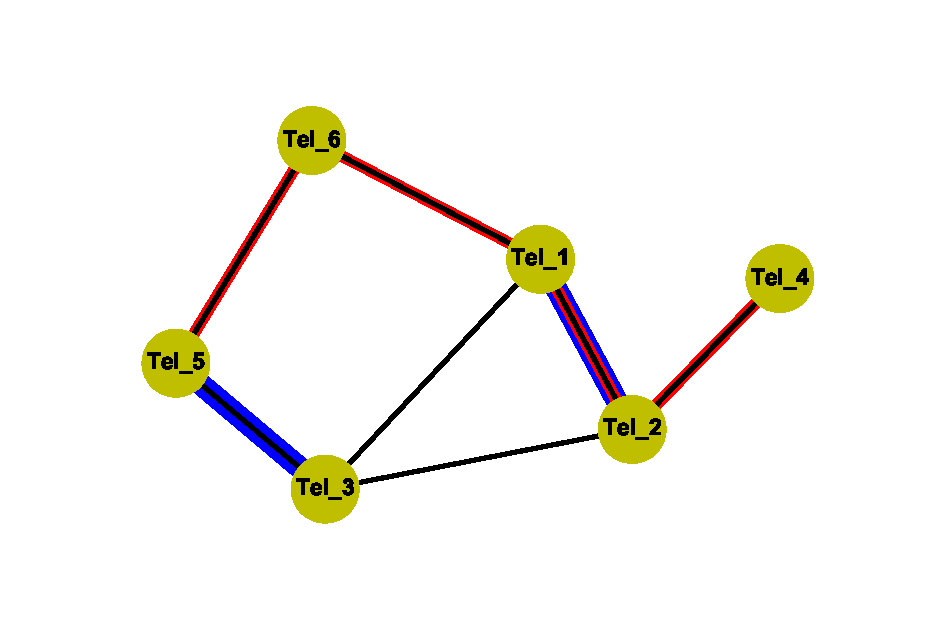
\includegraphics[scale=0.7]{Graf8.eps}\\
\caption{Multigrafo no dirigido cíclico, donde las aristas de diferentes colores representan la existencia de las llamadas con distinta duración}
\end{center}
\end{figure}
\section{Multigrafo no dirigido reflexivo}
Partiendo del ejemplo de la sección 3 se pretende construir un grafo más informativo a la hora de su análisis, por lo que se le agrega como arista (el hecho que las relaciones sexuales mantenidas fueran dentro de una relación formal). Este grafo se muestra en la figura 9.
\begin{center}
\lstinputlisting[language=Python]{grafo9.py}
\end{center}
\begin{figure}[h]
\begin{center}
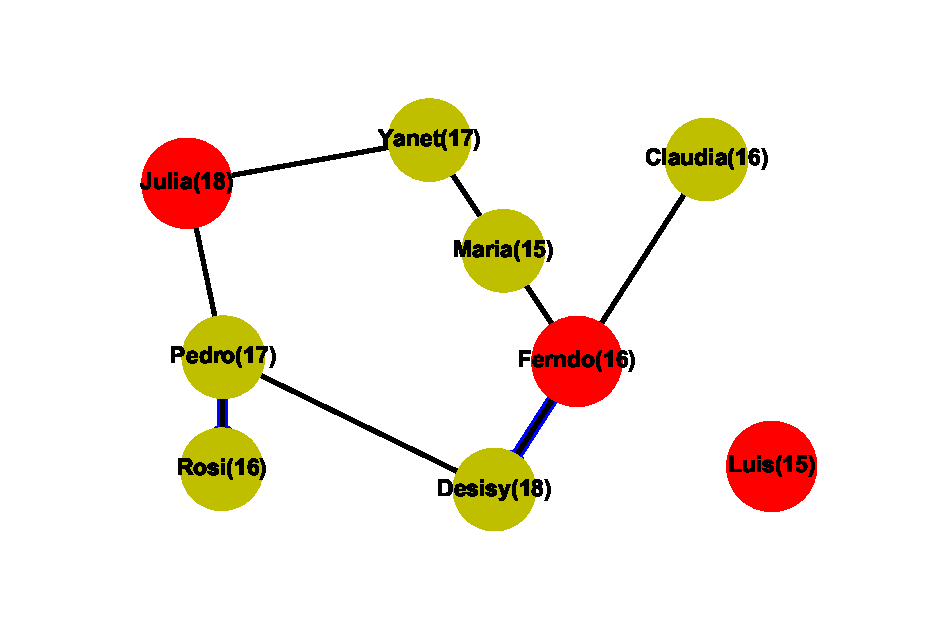
\includegraphics[scale=0.7]{Graf9.eps}\\
\caption{Multigrafo no dirigido reflexivo, donde las aristas de diferentes colores representan la existencia de una relación formal entre los individuos y los vértices de color rojo representa los vértices con aristas reflexivas}
\end{center}
\end{figure}
\section{Multigrafo dirigido acíclico}
Considerando que se quiere trazar las diferentes rutas (teniendo en cuenta el sentido de los mimas) que llevan de una provincia a otra en Cuba (Pinar del Río, Artemisa, La Habana, Mayabeque, Matanza, Cienfuegos, Villa Clara). Tomando como vértices las provincias y como aristas las carreteras que las unen, como muestra la figura 10.
\begin{center}
\lstinputlisting[language=Python]{grafo10.py}
\end{center}
\begin{figure}[h]
\begin{center}
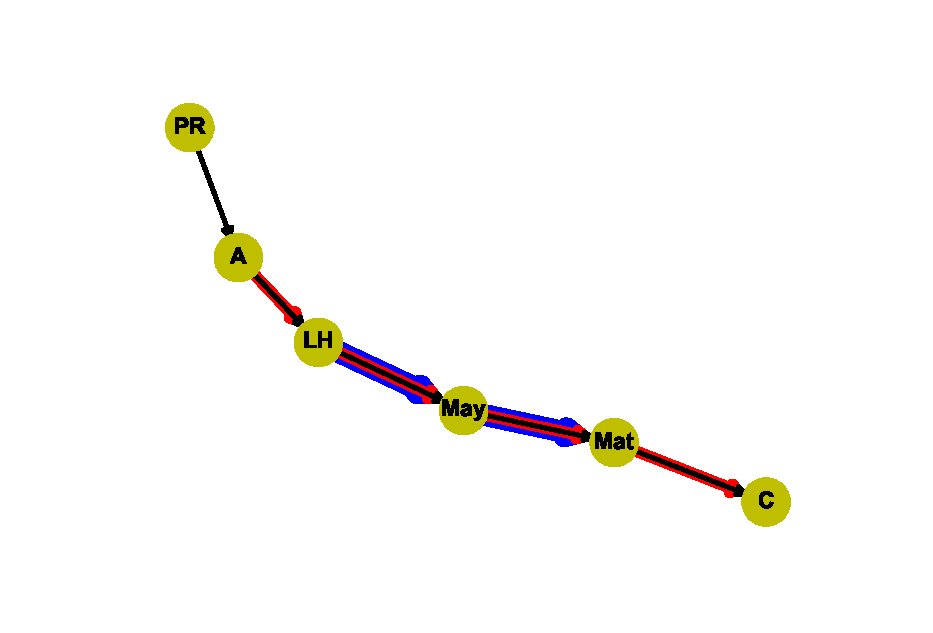
\includegraphics[scale=0.7]{Graf10.eps}\\
\caption{Multigrafo dirigido acíclico, donde las aristas de diferentes colores representan las existencia de mas de una ruta entre las diferente provincias}
\end{center}
\end{figure}

\section{Mltigrafo dirigido cíclico}
"En el caso particular de que las redes reflejen una realidad social, los nodos pueden representar personas o entidades relacionadas con sus contextos, y las conexiones representarán relaciones sociales existentes entre ellos (amistad, parentesco, membresía, afinidad, etc.). A pesar de que intuitivamente las redes sociales se asemejan a los grafos matemáticos, es más habitual que en ellas se trabaje con distintos tipos de relaciones"\cite{gf3} por lo que es necesario la utilización de multígrafos, que es la herramienta que contempla más de una relación entre dos nodos, con esto ganamos mayor riqueza en los datos a analizar.\linebreak 
Por ejemplo, tenemos un grupo de personas que laboran en un departamento de Informática y se hace una encuesta donde se les pide que marque cuales de tres sentimientos (respeto, afinidad, rechazo) sienten por sus compañeros de trabajo, como muestra la figura 11.

\begin{center}
\lstinputlisting[language=Python]{grafo11.py}
\end{center}
\begin{figure}[h]
\begin{center}
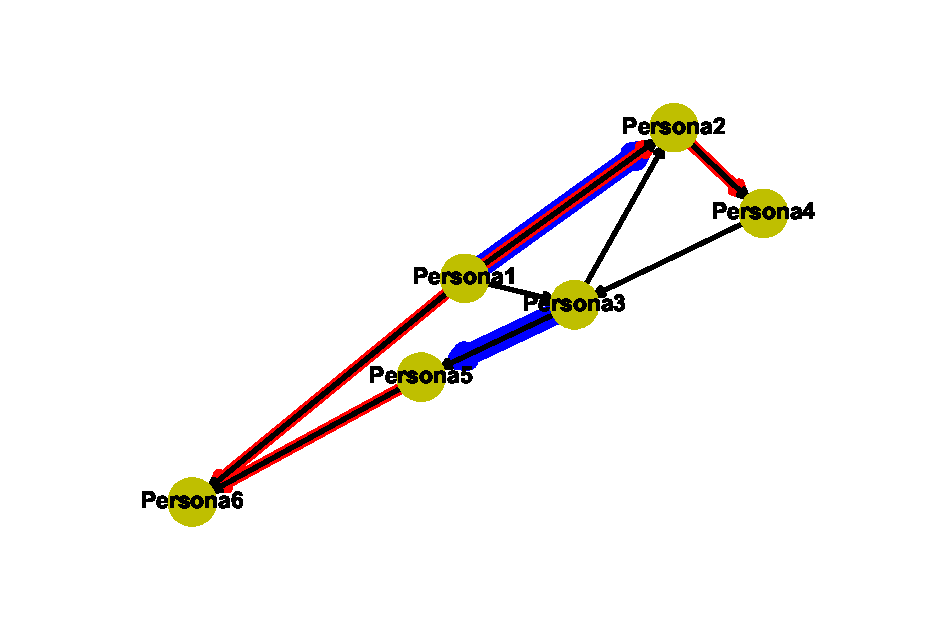
\includegraphics[scale=0.7]{Graf11.eps}\\
\caption{Mltigrafo dirigido cíclico, donde las aristas de diferentes colores representan las existencia de más de una opinión sobre sus compañeros}
\end{center}
\end{figure}

\section{Multigrafo dirigido reflexivo}
Una de las aplicaciones de estos grafos es en el modelado del funcionamiento de una maquina de estados. 
Por ejemplo, se desea modelar un grafo que represente el funcionamiento de una maquina muy sencilla de golosinas, que responde a las siguientes reglas:
\begin{itemize}
\item[1] Cada golosina vale \$ 0.25.
\item[2] La máquina acepta sólo monedas de  \$0.10 y de \$ 0.05.
\item[3] la máquina NO da vuelto.
\end{itemize}
Para modelar el grafo, debemos considerar distintos “estados de dinero ingresado”, y como se va pasando de uno a otro. Por ejemplo, si en un momento tenemos ingresados 5 centavos, y agregamos 5 centavos más, pasamos a otro estado, que es el mismo que si hubiésemos ingresado 10 centavos al principio. Llamemos A, B, C, D, E y F a los estados que representan 0, 5, 10, 15, 20, 25 centavos ingresados respectivamente. Las transiciones de un estado a otro se harán por ingreso de 5 o 10 centavos, o al presionar el botón para obtener los caramelos (G).Como se muestra en la imagen 12. 
\begin{center}
\lstinputlisting[language=Python]{grafo12.py}
\end{center}
\begin{figure}[h]
\begin{center}
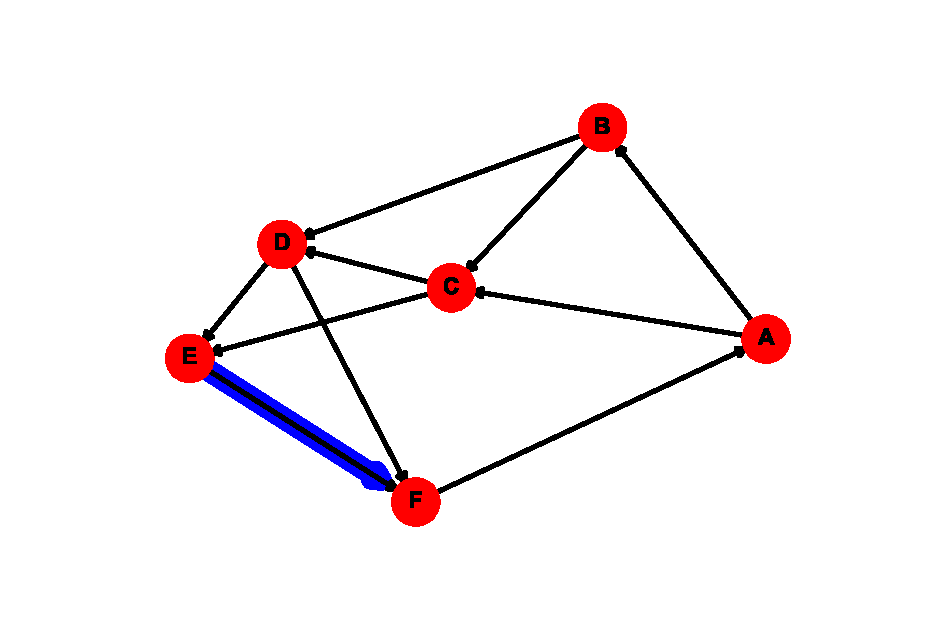
\includegraphics[scale=0.7]{Graf12.eps}\\
\caption{Mltigrafo dirigido reflexivo, donde las aristas de diferentes colores representan las existencia de mas de una forma de pasar de un estado a otro}
\end{center}
\end{figure}

\bibliography{tarea1}
\bibliographystyle{plain}
\end{document}
